\documentclass[a4paper, 10, conference]{ieeeconf}  % Comment this line out if you need a4paper

\IEEEoverridecommandlockouts                              % This command is only needed if 
                                                          % you want to use the \thanks command

\overrideIEEEmargins   
\usepackage[table]{xcolor} 
\usepackage{tikz}							% programmatically defines drawings
\usetikzlibrary{arrows}							% configures arrow tips
\usetikzlibrary{arrows.meta}					% necessary to draw graphs
\usetikzlibrary{positioning}
\usepackage[font=small,labelfont=bf]{caption}
\usepackage{multirow,relsize}
\usepackage{cite}
\usepackage{amsmath,amssymb,amsfonts}
\usepackage{algorithmic}
\usepackage{graphicx}
\usepackage{textcomp}
\usepackage[strings]{underscore}
\usepackage{adjustbox}
\usepackage{footnote}
\usepackage[super]{nth}
\usepackage{amsmath,fancyhdr}
\usepackage{scalefnt}


\pagestyle{fancy}
\renewcommand{\headrulewidth}{0pt}
\cfoot{\thepage}



\title{\LARGE \bf
Toward Cybersecurity of UAS operations under ``Specific" category
}

\author{Trung Duc Tran$^{1}$$^{2}$, Jean-Marc Thiriet$^{1}$, Nicolas Marchand$^{1}$, Amin El Mrabti$^{2}$% <-this % stops a space
	\thanks{*This work was supported by SOGILIS Company, Corresponding author: {\tt\small Trung-Duc.Tran@gipsa-lab.fr}}% <-this % stops a space
	\thanks{$^{1,}$Univ. Grenoble Alpes, CNRS, Grenoble INP, GIPSA-lab, 38000 Grenoble, France}%
	\thanks{$^{2}$SOGILIS Company, 38000 Grenoble, France}
}


\begin{document}

\bibliographystyle{IEEEtran}


\maketitle


%%%%%%%%%%%%%%%%%%%%%%%%%%%%%%%%%%%%%%%%%%%%%%%%%%%%%%%%%%%%%%%%%%%%%%%%%%%%%%%%
\begin{abstract}
 Nowadays, the increasing number of UAS operations raises the public concerns on cybersecurity issues. Therefore, it requires a methodology to address these issues during the UAS development. The Specific Operation Risk Assessment (SORA) is a risk assessment methodology developed by Joint Authorities for Rulemaking on Unmanned Aircraft System (JARUS). This methodology is endorsed by European Union Aviation Safety Agency (EASA) as an acceptable means to fulfill the requirements of EU regulation related to UAS operations under Specific category. The original SORA methodology focus on Safety risk scenarios only, which relate to unintentional threats and the harms to people's life. In this paper, we introduce our solution to extend the methodology toward cybersecurity aspects. The extended methodology concerns risk scenarios relating to intentional digital threats and some other harms (e.g privacy violation, damage to critical infrastructure). A part of this solution is developed and is presented in this paper.  
\end{abstract}


%%%%%%%%%%%%%%%%%%%%%%%%%%%%%%%%%%%%%%%%%%%%%%%%%%%%%%%%%%%%%%%%%%%%%%%%%%%%%%%%
\section{INTRODUCTION}
\subsection{Context}
For several years, the civil Unmanned Aircraft Systems (UAS) have become more and more popular with many applications such as aerial photography, goods transportation, surveillance, etc \cite{vattapparamban_drones_2016}. However, the lack of human observation, communication capacities, and protection makes UAS a good target for cyber attacks. Therefore, the risk related to the cybersecurity of UAS should be assessed and taken into account in the early phase of UAS development.

\begin{figure}[!ht]
	\centering
	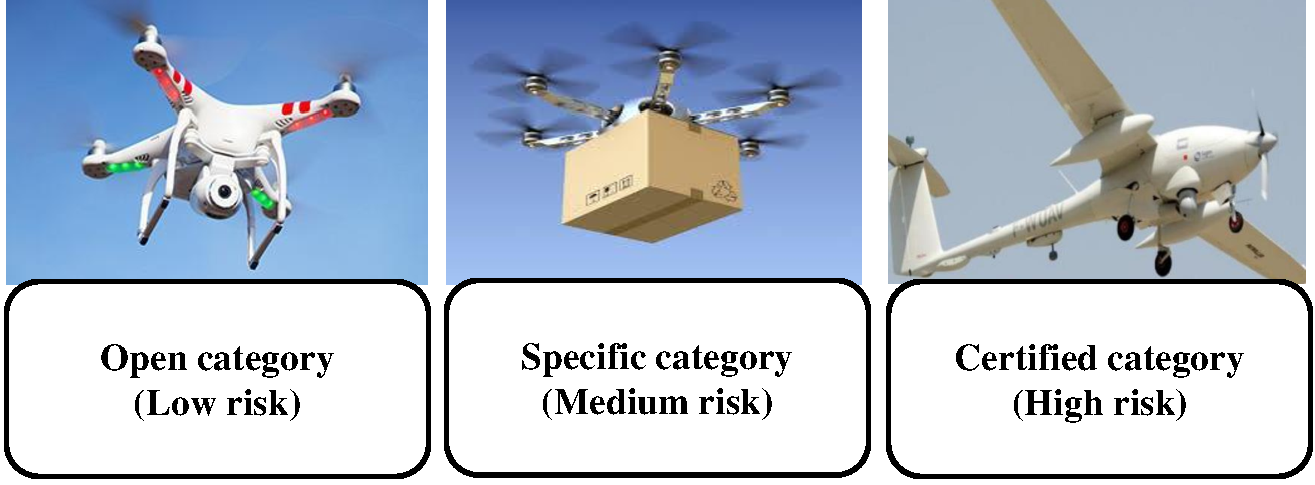
\includegraphics[width=3.3 in]{image/3categories.pdf}
	\caption{Three categories of UAS operations \textcolor{red}{A refaire - Nico}}
	\label{fig: riskscenario}
\end{figure}    

To deal with the progressive increase in the number of UAS operations, the European Aviation Safety Agency (EASA) classified UAS operations into three categories from Low to High risk level: Open, Specific and Certified \cite{A-NPA2015}. It is forecast that most of commercial UASs will operate under Specific Category \cite{EDOS2016}. In this category, we could expect the operation of large drones flying above populated areas, out of the visual line of sight of the pilot and sharing airspace with manned aircraft. These operations could pose significant harms to the people overflown and the manned aircraft, specially in case of a cyber attack. For these reasons, our works presented in this paper focus on the cybersecurity issue of operations under the Specific Category.



\subsection {Related works and contribution}

Regarding UAS applications, there are a lot of researches on cybersecurity breaches. Vattapparamban et al. experimented with several hijack attacks against small UASs by exploiting the vulnerabilities of their WiFi communication \cite{vattapparamban_drones_2016}. Heiges et al. \cite{heiges_how_nodate} experimented with an injection attack on an autopilot to reroute an Unmanned Aircraft (UA). Javaid et al. simulated GPS Jamming and GPS Spoofing attacks by using UAVSim \cite{10.1177/0037549716685874}. Davidson et al. argued that the optical flow sensors used for navigation represent a vector for adversarial control and demonstrated this argument with a real UAV \cite{198490}. The researches in individual security breaches are important because they help us anticipate the potential attacks against UAS operations and possible countermeasures. However, it is still a lack of researches on the decision-making process which helps to analyze globally the cybersecurity environment and balancing the operation performance vs. the economic cost of implementing countermeasures. 

In the other industrial domains, there are standards and methodologies which provide different guidances for risk assessment related to cybersecurity. For Industrial Automation and Control Systems (IACS), \textbf {IEC62443} standard guides on assessing risks and provides a list of requirements that need to meet during designing and implementing a secured system \cite{CSIAC-2016}. In the automobile domain, \textbf{E-safety Vehicle Intrusion proTected Applications (EVITA)}\cite{article-EVITA_2007} \cite{evita23} is a methodology dedicated to the cybersecurity of an on-board network, which has many common points with UAS (sensors, gps, actuators, control system etc.). This methodology aims to analyze cybersecurity breaches, define requirements and verify cyber-security solutions. In the aeronautic domain, \textbf{DO326/ED203} adds a new cybersecurity brick on the current manned aircraft development processes, which traditionally focuses on the safety \cite{ED202}. However DO326/ED203 and manned aircraft development processes are considered too costly for most of UAS operations, especially under the Specific category \cite{A-NPA2015}. 

Besides the methodologies and standards widely accepted in the industry, there are a lot of researches proposing the new risk assessment methodologies related to cybersecurity. Some of such methodologies are extended versions of existing risk assessment methodologies for safety \cite{bondavalli_security_2014, abdo:tel-01829574, jonsson_integrated_1998, 7490632, kriaa_joint_nodate}. Schmittner developed the FMVEA (Failure Mode, Vulnerabilities  and  Effects Analysis) method  based on the traditional FMEA (Failure  Mode  and  Effect  Analysis)\cite{bondavalli_security_2014}. The authors extended the original risk model to cover new incidents original from attacks and introduced new parameters to evaluate the attack likelihoods. Abdo et al.\cite{abdo:tel-01829574} treated the cybersecurity and safety issues for critical infrastructures in the same risk assessment process. The authors developed an approach to represent exhaustively risk scenarios and evaluate the likelihoods based on the Bow-tie model, which is commonly used in safety methodologies (for example in the SORA methodology \cite{dlr121660}). Xu et al. \cite{7490632} proposed a methodology to identify and analyze systematically cybersecurity risks based on Fault Tree Analysis and Hazard Analysis methods commonly used for safety in the aerospace industry.

To the best of our knowledge,  the most common risk assessment methodology in the UAS domain is \textbf{Specific Operation Risk Assessment (SORA)}, which is endorsed by European Aviation Safety Agency (EASA) as an acceptable means to fulfill the requirements of the EU regulations related to UAS. However, at this moment, the methodology focuses on only the safety aspect and ignores the cybersecurity aspect\cite{SORAV1}. Therefore, we introduce a solution to extend the SORA methodology to take into account cybersecurity aspects of UAS operation under the Specific category. The expected result of the application of the extended method is a list of cybersecurity and safety objectives which need to be addressed at the beginning of the UAS development process. 

The remaining of this document is organized as follows. The concept of the SORA methodology is then given in Section \ref{sec:concept}. A solution to extend the methodology to cybersecurity issues is given in Section \ref{sec:frame}. An extension of SORA methodology with the privacy harm is given in Section \ref{sec:newharm}. We conclude our works and present our perspective on the future works in Section \ref{sec:con}


\section{General concept of the SORA methodology} \label{sec:concept}

 Under the Specific category, to gain flight permission, operators (a person or a organization deploys and control the drone) have to demonstrate the safety of operation to aviation authorities by carrying out a risk assessment. One acceptable means to carry out this risk assessment is the  Specific Operations Risk Assessment (SORA) methodology proposed by a group of experts from the National Aviation Authorities - Joint Authorities for Rulemaking on Unmanned Systems (JARUS) \cite{EASA_AMC, EASA_SORA}. SORA is a holistic and operation-centric methodology \cite{dlr121660}.  It focuses on analyzing qualitatively consequences of safety issues related to an intended operation and then to determine the safety objectives (in training, system performance, organization, development), which need to be met to gain an  approval. From the point of view of manufacturers (who design and develop UAS), the SORA methodology could be used to determine safety feature that their designs need to reach to targeted operations under Specific category. In this section, we explain the general concept of the methodology including two parts: (1) risk model, (2) assessment process.

\subsection{Risk model}

 At this moment, the SORA methodology basically considers only risks of harms to a person's life: ``fatal injuries to third parties on ground", ``fatal injuries to third parties in air". To illustrate the risk scenarios related to these harms (or how these harms could happen), the methodology provides a risk model as shown in Figure \ref{table: riskscenario}. This risk model includes three major segments: Harms, Hazard, Threats. The harms are in the right part of the model. The direct causes of these harms is a generic hazard ``UAS operation out of control" shown in the center of the model. This hazard is defined as an operation being conducted outside of the operator's intention (e.g the aircraft flies outside of visual observation of the pilot in a Visual Line Of Sight operation). The hazard could be caused by several threats which are grouped into categories in the left part of the model. Because SORA methodology considers only the safety aspect but not the security aspect, only unintentional threats are represented in the model. However, according to the authors, this model could be extended to cover more risk scenarios \cite{SORAV1}.
 
 To mitigate the above risks, several means of mitigation should be applied. There are two types of means of mitigation: 
\begin{itemize}
	\item Harm barrier, which mitigates the likelihood of harms after an occurrence of hazard (e.g. parachute, plan to save the victim on the ground). The harm barriers are pre-defined by operators/manufactures and are analyzed during the risk assessment. 
	\item Threat barrier, which mitigates the likelihood of ``UAS operation out of control" caused by considered threats. For each category of threat, different threat barriers will be determined at the end of risk assessment under the form of Operation Safety Objective (OSO). Each OSO is detailed in three levels of robustness (Low, Medium, High). An example of OSO is that ``the UAS is developed to authority recognized design standards"\cite{Annex_E_SORA}. At low robustness level  of this OSO, the applicant should only declare the required standards are achieved. Meanwhile at the high robustness level, the applicant has to provide supporting evidence (such as analysis, simulation), which will be valided by a competent third party.  
\end{itemize}

%\begin{figure}[!ht]
%	\centering
%	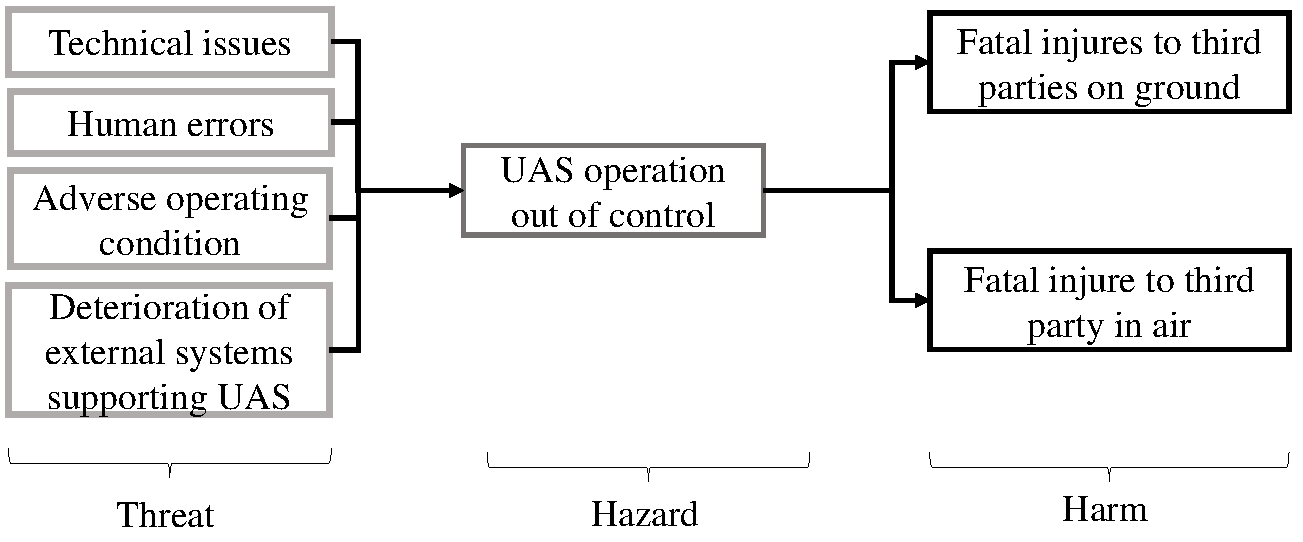
\includegraphics[width=3.3 in]{image/Bow-tie_model.pdf}
%	\caption{Risk model de the SORA methodology \textcolor{red}{A refaire - Nico}}
%	\label{table: riskscenario}
%\end{figure}  
\begin{figure}[!ht]
    \begin{center}\vskip-2mm
	   	\resizebox{.95\columnwidth}{!}{%
	   	    \relsize{1.2}% !TEX root = ../main.tex
% Graphic for TeX using PGF
% Title: /Applications/Dia.app/Diagramme1.dia
% Creator: Dia v0.97.2
% CreationDate: Thu Feb 27 13:32:45 2020
% For: marchann
% \usepackage{tikz}
% The following commands are not supported in PSTricks at present
% We define them conditionally, so when they are implemented,
% this pgf file will use them.
\ifx\du\undefined
  \newlength{\du}
\fi
\setlength{\du}{13\unitlength}
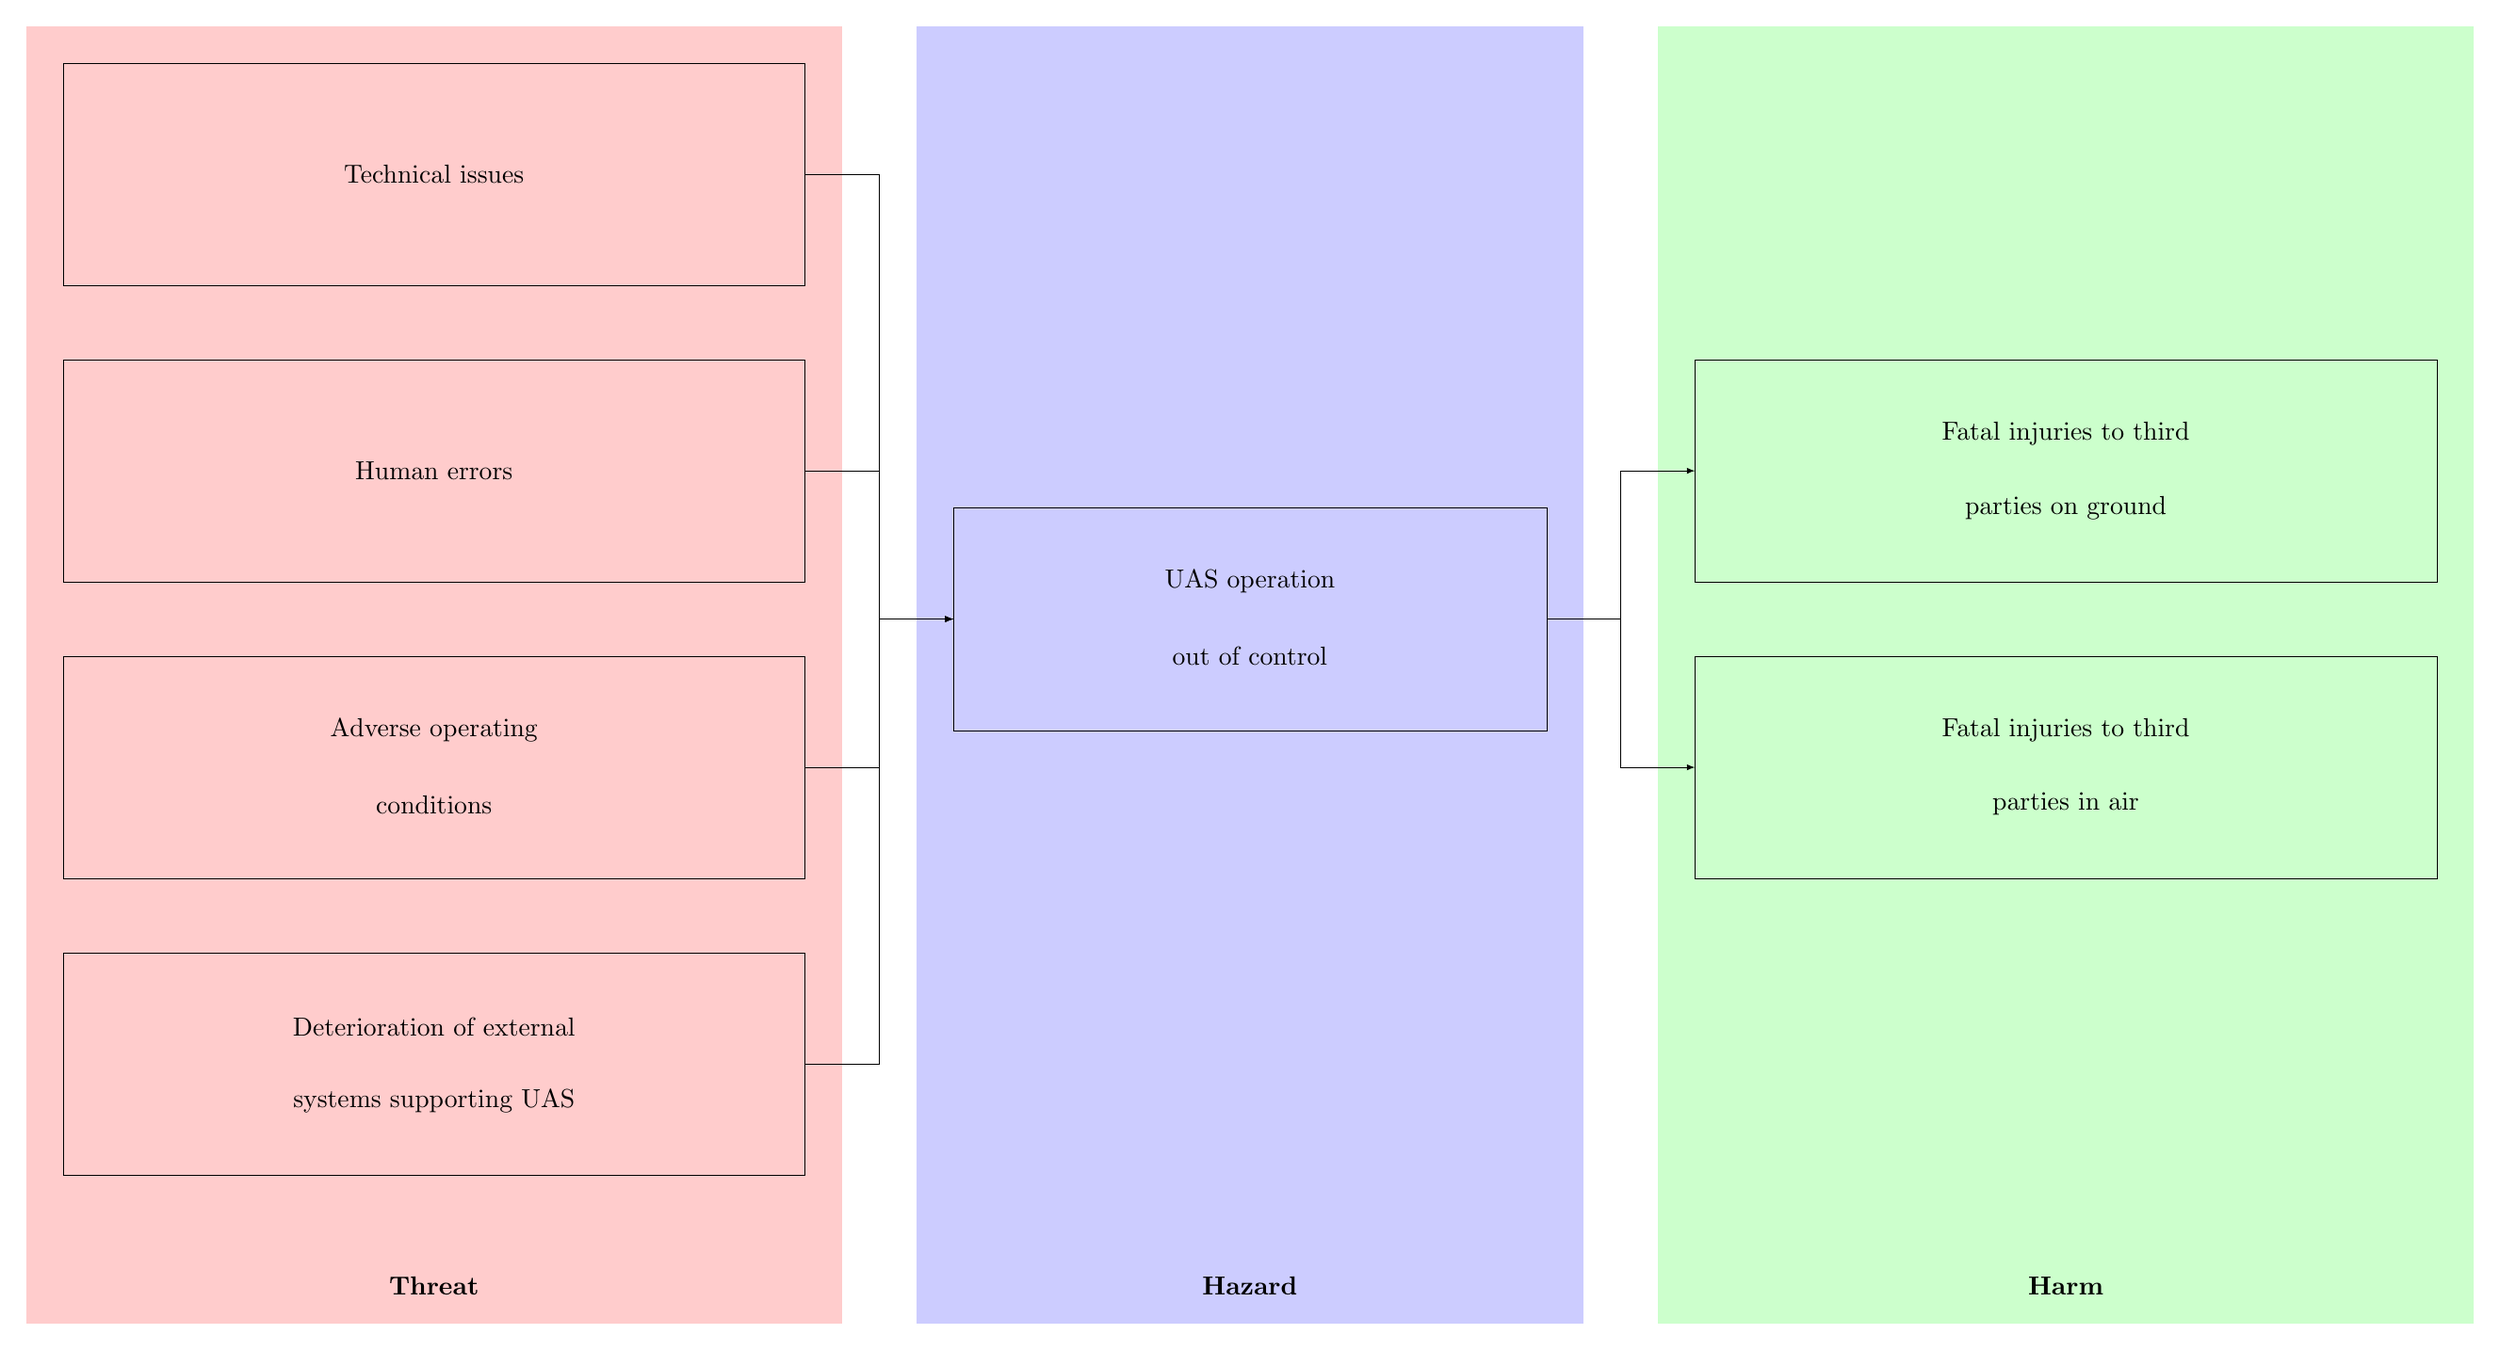
\begin{tikzpicture}
\pgftransformxscale{1.000000}
\pgftransformyscale{-1.000000}
\pgfsetlinewidth{0.100000\du}

%%%%%%%%%%%%%%%% Boites %%%%%%%%%%%%%%
\fill[color=red!20] (-.5\du,-.5\du)--(-.5\du,17\du)--(10.5\du,17\du)--(10.5\du,-.5\du)--cycle;
\node at (5\du,16.5\du){\bf Threat};

\pgfsetstrokecolor{black}
\draw (0\du,0\du)--(0\du,3\du)--(10\du,3\du)--(10\du,0\du)--cycle;
\node at (5\du,1.5\du){Technical issues};
\draw (0\du,4\du)--(0\du,7\du)--(10\du,7\du)--(10\du,4\du)--cycle;
\node at (5\du,5.5\du){Human errors};
\draw (0\du,8\du)--(0\du,11\du)--(10\du,11\du)--(10\du,8\du)--cycle;
\node at (5\du,9\du){Adverse operating};
\node at (5\du,10\du){conditions};
\draw (0\du,12\du)--(0\du,15\du)--(10\du,15\du)--(10\du,12\du)--cycle;
\node at (5\du,13\du){Deterioration of external};
\node at (5\du,14\du){systems supporting UAS};


\fill[color=blue!20] (11.5\du,-.5\du)--(11.5\du,17\du)--(20.5\du,17\du)--(20.5\du,-.5\du)--cycle;
\node at (16\du,16.5\du){\bf Hazard};
\draw (12\du,6\du)--(12\du,9\du)--(20\du,9\du)--(20\du,6\du)--cycle;
\node at (16\du,7\du){UAS operation};
\node at (16\du,8\du){out of control};

\fill[color=green!20] (21.5\du,-.5\du)--(21.5\du,17\du)--(32.5\du,17\du)--(32.5\du,-.5\du)--cycle;
\node at (27\du,16.5\du){\bf Harm};
\draw (22\du,4\du)--(22\du,7\du)--(32\du,7\du)--(32\du,4\du)--cycle;
\node at (27\du,5\du){Fatal injuries to third};
\node at (27\du,6\du){parties on ground};
\draw (22\du,8\du)--(22\du,11\du)--(32\du,11\du)--(32\du,8\du)--cycle;
\node at (27\du,9\du){Fatal injuries to third};
\node at (27\du,10\du){parties in air};



%%%%%%%%%%%%%%% Flèches %%%%%%%%%%%%%%%
\pgfsetbuttcap
{
\pgfsetarrowsend{latex}
{\pgfsetcornersarced{\pgfpoint{0.000000\du}{0.000000\du}}
\pgfsetmiterjoin
\pgfsetstrokecolor{black}
\draw (10\du,1.5\du)--(11\du,1.5\du)--(11\du,7.5\du)--(12\du,7.5\du);
\draw (10\du,5.5\du)--(11\du,5.5\du)--(11\du,7.5\du)--(12\du,7.5\du);
\draw (10\du,9.5\du)--(11\du,9.5\du)--(11\du,7.5\du)--(12\du,7.5\du);
\draw (10\du,13.5\du)--(11\du,13.5\du)--(11\du,7.5\du)--(12\du,7.5\du);
}}

\pgfsetbuttcap
{
\pgfsetarrowsend{latex}
{\pgfsetcornersarced{\pgfpoint{0.000000\du}{0.000000\du}}
\pgfsetmiterjoin
\pgfsetstrokecolor{black}
\draw (20\du,7.5\du)--(21\du,7.5\du)--(21\du,9.5\du)--(22\du,9.5\du);
\draw (20\du,7.5\du)--(21\du,7.5\du)--(21\du,5.5\du)--(22\du,5.5\du);
}}

\end{tikzpicture}
}
	\end{center}\vskip-2mm
	\caption{Risk model de the SORA methodology}
	\label{table: riskscenario}
\end{figure}


 In the next part, we explain the assessment process of the SORA methodology based on the above risk model in both quantitative and qualitative approaches.

\subsection{Assessment process}

\subsubsection{Quantitative approach}
Traditionally, the risk assessment process requires to analyze two parameters of risk: likelihood and severity. However, the risks in the SORA methodology is tied to only likelihood parameters \cite{SORAV1} because the methodology basically focuses on only risks of harms to person's life. The severity of these harms could be considered as extremely high. In other words, the safety objectives will be determined to maintain the likelihood of each harm under the acceptable value ( $10^{-6}$ fatal injuries per flight hour, equivalent to a manned aircraft operation\cite{SORAV1}). The likelihood of these harms is decomposed into individual components as shown in Figure \ref{figure: likelihood estimation}. 

 \begin{figure}[!ht]
 	\centering
 	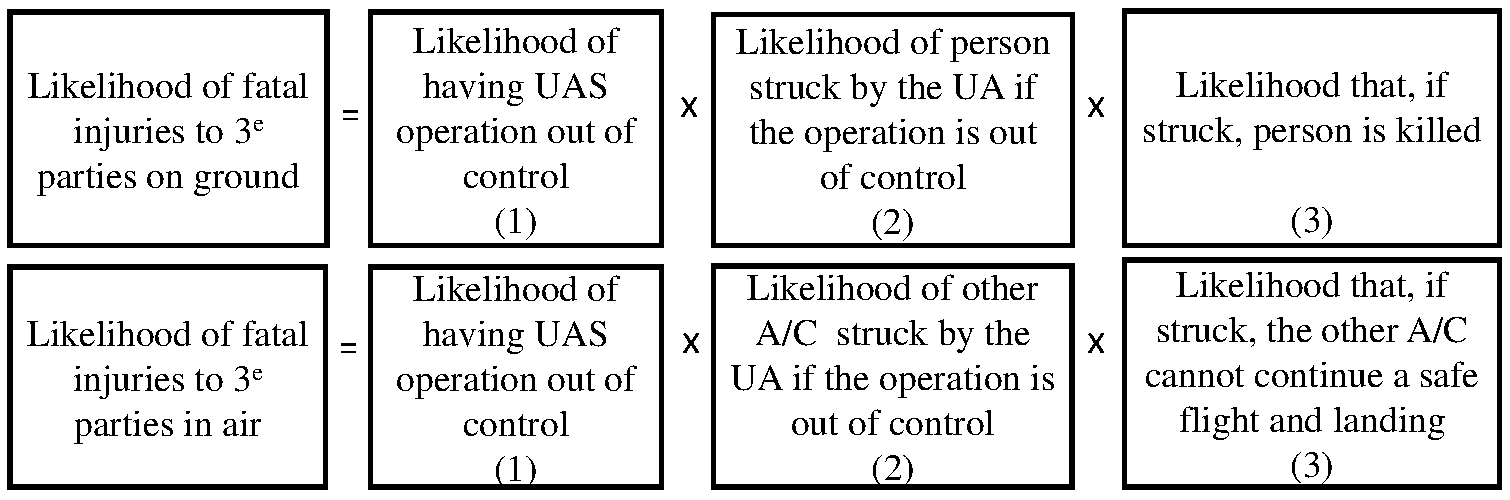
\includegraphics[width=3.4 in]{image/likelihood_estimation.pdf}
 	\caption{Likelihood of fatal injuries on ground and in air \cite{SORAV1} \textcolor{red}{A refaire - Nico}}
 	\label{figure: likelihood estimation}
 \end{figure}  
 
The component 1 of each equation, ``likelihood of having UAS operation out of control" is mainly affected by the threats and threat barriers \cite{SORAV1}. The combination of component 2 and component 3 in each equation represents the likelihood of harms in case of having UAS operation out of control, which could be evaluated by analyzing the nature of operation under consideration (e.g location, altitude, kind of operation, harm barriers in place). Under the above assumption, the general concept of this methodology in the quantitative approach could be explained as follows:
  \begin{itemize}
  	\item \textbf{Objective:} Given a UAS operation, we need to maintain the likelihood of each harm under acceptable value: $10^{-6}$ fatal injuries per flight hour.
  	\item \textbf{Firstly}, we collect the information on the intended operation of the UAS such as operation area, operation mode, pilot, weight of UA. This activity is called Concept Of Operations (CONOPS) description. The form of a CONCOPS description is provided in Annex A of the SORA methodology.
  	\item \textbf{Secondly}, we estimate the likelihood that the harms occur in case of ``UAS operation out of control" based on collected information (e.g. $10^{-4}$ fatal injuries on ground per hazard and $10^{-3}$ fatal injuries in air per hazard).
  	\item \textbf{Thirdly}, from the estimated values above, we calculate an \textbf{acceptable} value for the likelihood of having UAS operation out of control ($10^{-2}$ hazard per flight hour from the first equation and $10^{-3}$ hazard per flight hour from the second one). The more critical value will be chosen as an objective needs to be reached (e.g $10^{-3}$ hazard per flight hour).
  	\item \textbf{Lastly}, based on the objective value of ``likelihood of having UAS operation out of control", the safety objectives with corresponding robustness will be defined. 
  \end{itemize}


\subsubsection{Qualitative approach}

The qualitative approach presented above is generally not realistic because of the lack of real data. Therefore, the SORA methodology proposes a qualitative approach based on the main ideas of the quantitative approach as shown in Figure \ref{figure: Simplified SORA process}. The qualitative approach could be explained as follows:
	 \begin{figure}[!ht]
		\centering
		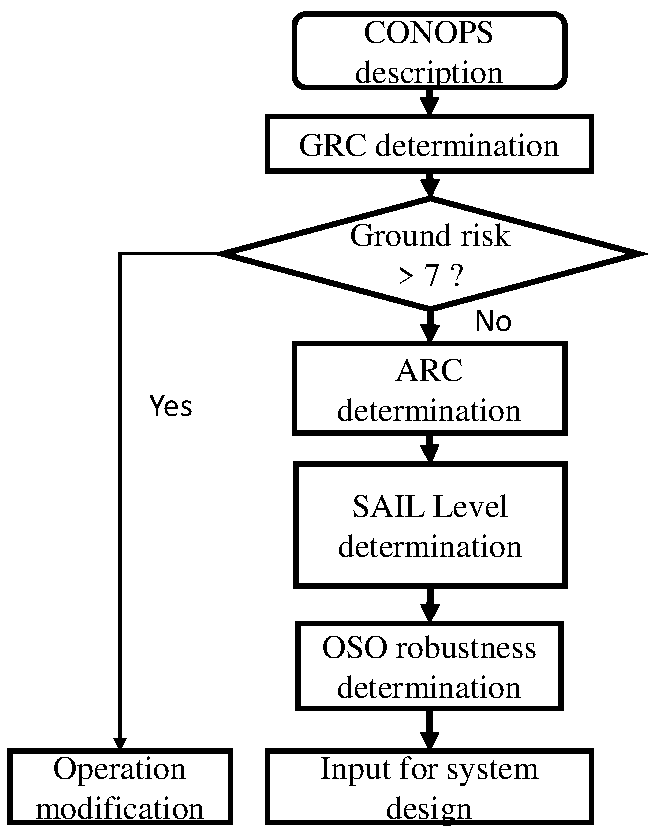
\includegraphics[width= 2.9 in]{image/original_workflow.pdf}
		\caption{Simplified risk assessment process \textcolor{red}{A refaire - Nico}}
		\label{figure: Simplified SORA process}
	\end{figure}  

   \begin{itemize}
   	\item \textbf{Objective:} Given a UAS operation, we need to maintain the likelihood of each harm at an acceptable level. 
   	\item \textbf{Firstly}, we collect the information on the intended operation (CONOPS description)
   	\item \textbf{Secondly}, we determine two qualitative factors: Ground Risk Class (GRC) and Air Risk Class (ARC). These factors represent qualitatively the likelihoods that the harms occur in case of UAS operation out of control. The GRC and ARC are determined based on the intrinsic characteristics of the operation such as operational area, attitude, weight of the UA and the availability of harm barriers. 
   	  
   	\item \textbf{Thirdly}, we determine two Specific Assurance and Integrity Levels (SAIL) values, which represent the level of confidence that the UAS operation will stay under control. One SAIL value corresponds to GRC and the other corresponds to ARC \cite{SORAV1}. Then, the higher SAIL value will be chosen as an objective to drive the required safety objectives. In the most recent version of the SORA methodology, these activities are simplified by using Table \ref {tab:SAIL determination}.
   	
   	\begin{table}[!ht]
   		\centering
   		%\begin{adjustbox}{width= 2.0 in}
	   		\begin{tabular}{|c|c|c|c|c|}
	   			\hline
	   			\multicolumn{5}{|c|}{SAIL Determination} \\ \hline
	   			\rowcolor[HTML]{C0C0C0} 
	   			& \multicolumn{4}{c|}{\cellcolor[HTML]{C0C0C0}ARC} \\ \hline
	   			\rowcolor[HTML]{C0C0C0} 
	   			GRC & a & b & c & d \\ \hline
	   			\cellcolor[HTML]{C0C0C0}$\leq2$ & I & II & IV & V \\ \hline
	   			\cellcolor[HTML]{C0C0C0}3 & II & II & IV & V \\ \hline
	   			\cellcolor[HTML]{C0C0C0}4 & III & III & IV & V \\ \hline
	   			\cellcolor[HTML]{C0C0C0}5 & IV & IV & IV & V \\ \hline
	   			\cellcolor[HTML]{C0C0C0}6 & V & V & V & V \\ \hline
	   			\cellcolor[HTML]{C0C0C0}7 & VI & VI & VI & VI \\ \hline
	   		\end{tabular}
   		%\end{adjustbox}
   		\caption{SAIL determination \cite{SORAV2} \textcolor{red}{A refaire - Nico}}
   		\label{tab:SAIL determination}
   	\end{table}
   
   	\item \textbf{Lastly}, we chose Operation Safety Objective (OSO) and their robustness level corresponding to the SAIL level of the operation. A list of all possible OSOs is provided in the annex E of SORA \cite{Annex_E_SORA}.
   \end{itemize}
   

In this section, we explained the original concept of the SORA methodology. It could be resumed as: (1) firstly, evaluate the critical level of a UAS operation based on the likelihood of harms in case of ``UAS operation out of control", (2) then determine threat barriers corresponding to the critical level of the operation. In the next section, we propose a solution to extend this methodology to cover cybersecurity aspect based on this concept.

\section{Solution to extend the SORA methodology toward cybersecurity}\label{sec:frame}

Our proposed solution consists of two parts which are called Harm Extension and Threat Extension. Harm Extension extends the risk scenarios under consideration with new harms; and completes the evaluation of critical level of a given UAS operation. Threat Extension extends the scenarios under consideration with new cyber security threats; and determines the corresponding threat barriers for a given UAS operation. The development of Harm Extension is now in process while Threat Extension has not been developed yet.
\begin{figure}[!ht]
	\centering
	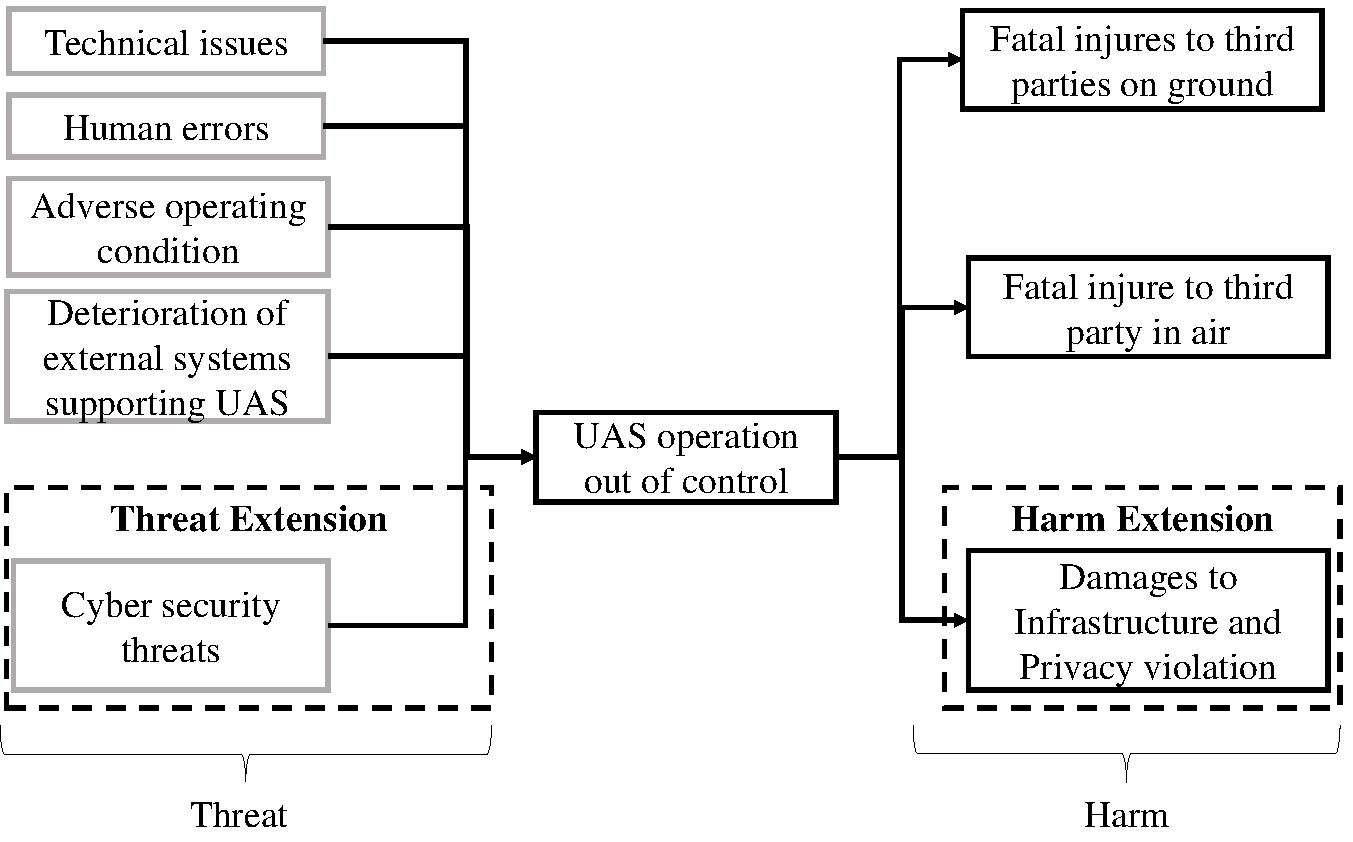
\includegraphics[width=3.3 in]{image/extended_SORA.pdf}
	\caption{Extended risk model \textcolor{red}{A refaire - Nico}}
	\label{figure: Extended risk model}
\end{figure}

In Harm Extension, we concern the harm-side of the risk model (see Figure \ref{figure: Extended risk model}). The classical SORA methodology concerns only the harms to person's life. However, besides the harms to person's life the public concerns also the other harms \cite{A-NPA2015, SORAV1,EASA_SORA,7383633} such as:  
\begin{itemize}
    \item \textbf{Privacy violation}: A UAS could have a small size, a long operational range and high performance on-board sensors; so it could intrude itself into private locations and collect information \cite{8490190}. That violates the privacy of the owner.  The privacy violation could be caused by a cyber attack or an error of the system. For example, police-operated UASs may frequently cross private properties on their way to an operational area. Under a cyber attack, the recorded video on the properties could be disclosed and then the privacy of the owners overflown could be violated.  
    
    \item \textbf{Physical damages to infrastructure}: It is supposed that a UA could fall down on critical infrastructures such as highway, electricity power line, nuclear plant. This harm relates to only some specific operations in which UAs fly near or over critical infrastructures.
    
    \item \textbf{Digital damage to infrastructure}: It is supposed that a UAS could become a security breach to critical infrastructure. For example, an attacker takes over control the UAS and uses it to attack an infrastructure via the connection between the UAS and the infrastructure.   
    
    
\end{itemize}
Therefore, they come to mind as important issues that should be taken into account in the extended methodology. In Harm Extension, our strategy to address the new harms includes four steps as follows:
\begin{enumerate}
	\item Chose a new harm that needs to be addressed
	\item Determine factors/characteristics of the UAS operation which have impact on the likelihood of the chosen harm.
	\item Establish formals or tables to evaluate qualitatively the likelihood based on the determined factors
	\item Extend ``SAIL determination'' step to cover the likelihood of the new harm. 
\end{enumerate}

In Threat Extension, we will concern the threat-side of the risk model. The potential cybersecurity threats need to be identified and grouped in new threat categories. In other words, this calls for a ``completed" taxonomy of cybersecurity threat related to a UAS operation. To illustrate the new scenarios, the new threat categories will be added into the harm-side of the risk model as shown in Figure \ref{figure: Extended risk model}. Corresponding to each new threat category, a list of possible threat barriers will be also established. For a given UAS operation, the new threat barriers are chosen in correspondence with the SAIL value. 

Harm Extension and Threat Extension could be separately developed and then could be integrated into one completed methodology. In the remaining of this paper, we focus on developing a part of Harm Extension related to privacy issue. 

\section{SORA methodology with privacy issue} \label{sec:newharm}

Nowadays, the privacy violation is one of the most concerned issues for public acceptance of UAS applications \cite{SORAV1, 7383633, Zhi2019}. Therefore, we consider it as important issue and address it firstly in our works. However, the general privacy is a very large term. It is difficult to define precisely \cite{Finn2013} and address this term at large, so we focus on only three aspects of this harm: (1) disclosure of personal information; (2) illegal personal surveillance; and (3) intrusion into a private location. The first aspect is illustrated in the works of Li et al. \cite{8685611}. The authors experimented a password-stealing attack by analysing the video captured by the drone.  The second aspect is mentioned in \cite{Johnvilla_privacy, 7883702, 7285023}. In these papers, the authors examined how the surveillance UAS application could impact on the privacy of people on the ground. Moreover, Park et al. \cite{7883702} and Babiceanu et al. \cite{7121232} proposed criteria for judging privacy violation of an UAS operation based on the quality of captured images/videos. The last aspect was addressed by Blank et al. \cite{8328983}. The authors proposed a mechanism to recognize private spaces during creating flight-paths and make sure that UAs would not fly over these private properties.

For the next, (A) we first analyse the likelihood of the privacy violation to determine the possible factors related to this harm, which could be used for the assessment. Then we propose extensions for the assessment process: (B) a new step named ``Privacy risk class (PRC) determination" to evaluate the likelihood of this harm in case of ``UAS operation out of control" and (C) an extension of the "SAIL determination" step (see Figure \ref{figure: New steps Ex1}). At the end, (D) a case-study is shown. 

  \begin{figure}[!ht]
   	\centering
   	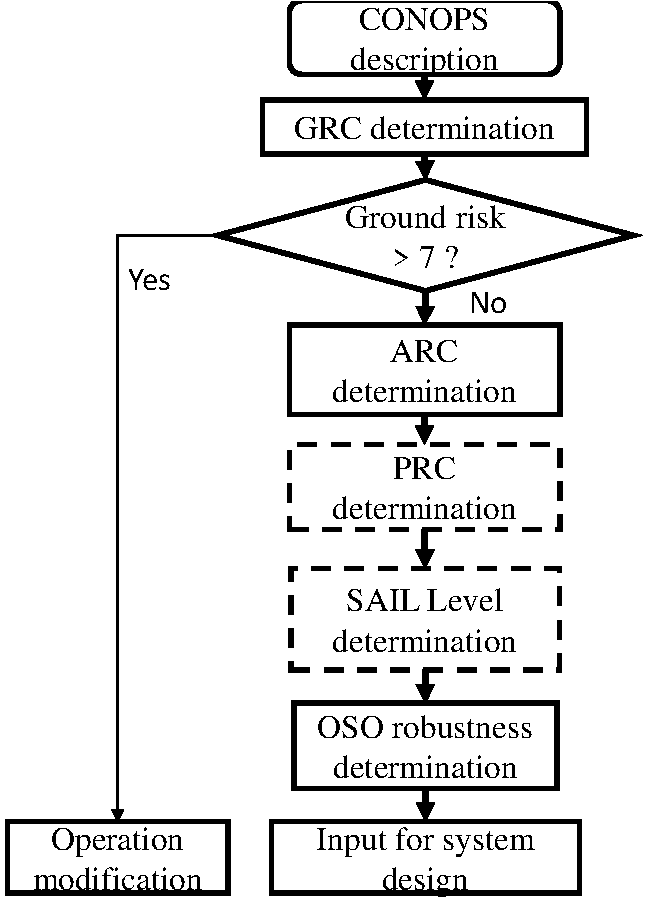
\includegraphics[width= 2.9 in]{image/Extended_Processs_in_module1.pdf}
   	\caption{New steps for Harm Extension \textcolor{red}{A refaire - Nico}}
   	\label{figure: New steps Ex1}
   \end{figure}  
   
\subsection {Likelihood of privacy violation}
With the privacy harm taken into account, the objective of risk assessment is extended to maintain that the likelihood of harms to privacy is also under certain acceptable level. Similar to the likelihood of harm to person's life, the one of the privacy harm could be decomposed as shown in Figure \ref{figure: new ham likelihood}. The combination of the two components (2) and (3) of this equation represents the likelihood that the privacy of third parties is violated after ''UAS operation out of control". 

\begin{figure}[!ht]
	\centering
	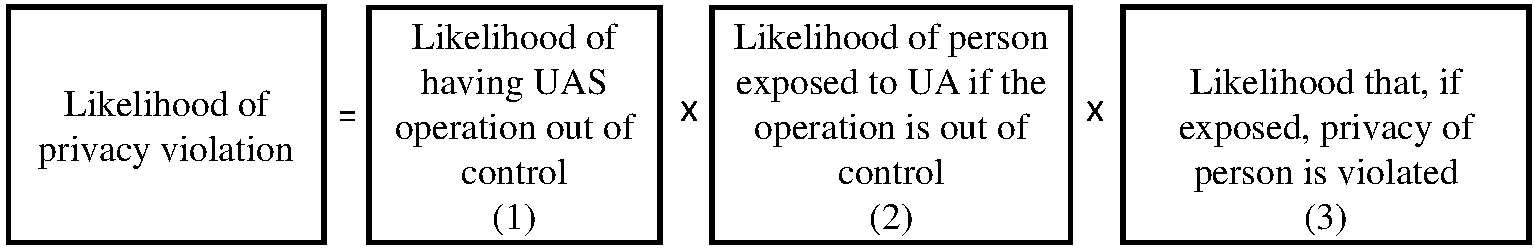
\includegraphics[width=3.3 in]{image/likelihood_of_privacy_violation.pdf}
	\caption{Likelihood of privacy violation \textcolor{red}{A refaire - Nico}}
	\label{figure: new ham likelihood}
\end{figure}

For a given operation, the likelihood of a person exposed to the UA (insides the sensing range or under the UA) depends on the nature of operation zone (urban zone vs. rural zone) and the type of operation (Beyond Light of Sight vs. Visual Light of Sight). In urban zones, the population density and the number of private locations is higher than in rural zones. Therefore, the likelihood of having a person or a private location exposed to a UA in an urban zone could be higher than in a rural zone. In a Beyond Light Of Sight (BLOS) operation, the operation range of UA is greater than in a Visual Light Of Sight (VLOS) operation. Therefore, the number of persons under or near a UA in a BLOS operation could be higher than in a VLOS operation. That's why  the likelihood of having a person or a private location exposed to UA could be higher in a BLOS operation than in a VLOS operation. 


 For a person exposed to the UA, the likelihood of privacy violation depends on the detail level of image collected by on-board camera. For example, if the photo taken by the UAS is at a too low resolution, the image of the person is not detailed enough to recognize her/his face so the likelihood of privacy violation is low. The detail level of image could be evaluated by the pixel density - the number of pixels in a captured image representing a meter on ground. To simplify the calculation we assume that the ground is flat. Therefore, for a UAS operation, the highest value of pixel density is reached when the camera direction is perpendicular to the ground as shown in Figure \ref{flat ground}. In this case, the pixel density is a function of the height above ground of UA (h), the resolution of the camera and the smallest angle of view of camera ($\alpha$) as follows:
 
  \[PD=\frac{\text{number  of  horizontal  pixels}}{2*h*\tan \frac{\alpha}{2}}(pixels/m)\]

\begin{figure}[!ht]
	\centering
	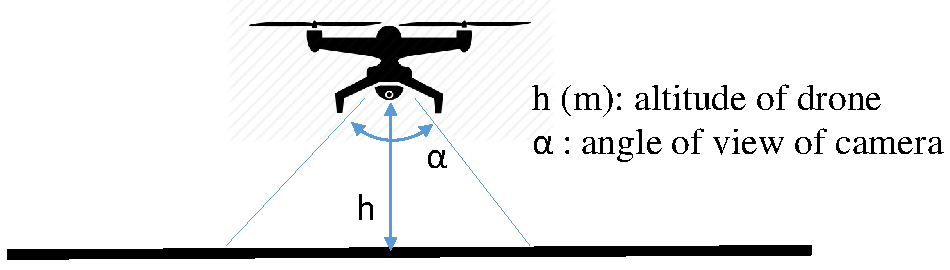
\includegraphics[width=3.2 in]{image/Maximum_pixel_density.pdf}
	\caption{Maximum pixel density position \textcolor{red}{A refaire - Nico}}
	\label{flat ground}
\end{figure}
Because there are common points related to privacy issue between UAS application and Closed-circuit television (CCTV) application \cite{7383633, 7883702, 7285023}, we adopt a classification of image detail levels introduced by the British Security Industry Association (BSIA) for CCTV application as shown in Table \ref{tab:Image quality classification}.

\begin{table}[!ht]
\centering
\begin{tabular}{|l|l|}
\hline
\textbf{Level of quality} & \textbf{Description}                                                                                                                             \\ \hline
Monitor (12.5pixels/m)     & \begin{tabular}[c]{@{}l@{}}Enable to view direction and speed of \\ movement of people, if knowing their \\ present.\end{tabular}                \\ \hline
Detect (25 pixels/m)      & Enable to reliably if a person is present                                                                                                        \\ \hline
Observe (62.5 pixels/m)   & \begin{tabular}[c]{@{}l@{}}Enable to characterize some details of an \\ individual\end{tabular}                                                  \\ \hline
Recognize (125 pixels/m)  & \begin{tabular}[c]{@{}l@{}}Enable to determine whether or not an \\ individual shown is the same as someone\\ they have seen before\end{tabular} \\ \hline
Identity (250 pixels/m)   & \begin{tabular}[c]{@{}l@{}}Enable identification of an individual \\ beyond a reasonable doubt.\end{tabular}                                     \\ \hline
Inspect (1000 pixels/m)   & Enable the identity of an individual                                                                                                             \\ \hline
\end{tabular}
\caption{Image detail classification \cite{BSIA2014} \textcolor{red}{A refaire - Nico}}
\label{tab:Image quality classification}
\end{table}

Based on this analysis, we define three intrinsic features of a UAS operation to evaluate the likelihood of privacy violation in case of ``UAS operation out of control":
\begin{itemize}
    \item Density of operational area: urban zone vs. rural zone
    \item Type of operation: BLOS vs. VLOS
    \item Level of detail of the captured image. 
   
\end{itemize}

Similar to harms introduced in the classical SORA methodology, the likelihood of privacy harm could be reduced by applying some harm barriers. In this extension, we address three types of harm barriers to mitigate the privacy harm: 

\begin{itemize}
    \item Privacy protection filters: these algorithms reduce unnecessary information that could violate the privacy of person from the video/image such as Blurring, Pixelization, Masking, Warping \cite{7285023}  
    \item Restriction on private space: the operator avoids make a flight path across a private space \cite{8328983}
    \item Operation-aware announcement to public: the public under observation of a UAS operation should be informed about it.
\end{itemize}

In the next parts of the paper, we provide the details of the  PRC determination step and the SAIL determination step.

\subsection {Privacy Risk Class determination step }
In this step, the likelihood of privacy violation in case of "UAS operation out of control" is represented qualitatively by the Privacy Risk Class (PRC) value. The intrinsic PRC value is determined based on the intrinsic features of operation as shown in Table \ref{intrinsic PRC}. 
\begin{table}[!ht]
\centering
\begin{tabular}{|
>{\columncolor[HTML]{EFEFEF}}l |l|l|l|l|}
\hline
\cellcolor[HTML]{9B9B9B}{\color[HTML]{000000} \textbf{\begin{tabular}[c]{@{}l@{}}Type of \\ operation\end{tabular}}} & \cellcolor[HTML]{9B9B9B}{\color[HTML]{000000} \begin{tabular}[c]{@{}l@{}}Rural \\ zone,\\ VLOS\end{tabular}} & \cellcolor[HTML]{9B9B9B}{\color[HTML]{000000} \begin{tabular}[c]{@{}l@{}}Rural \\ zone,\\ BLOS\end{tabular}} & \cellcolor[HTML]{9B9B9B}{\color[HTML]{000000} \begin{tabular}[c]{@{}l@{}}Urban \\ zone,\\ VLOS\end{tabular}} & \cellcolor[HTML]{9B9B9B}{\color[HTML]{000000} \begin{tabular}[c]{@{}l@{}}Urban \\ zone,\\ BLOS\end{tabular}} \\ \hline
\textbf{\begin{tabular}[c]{@{}l@{}}Image detail\\ level\end{tabular}} &  &  &  &  \\ \hline
Monitor & A & B & C & C \\ \hline
Detect & B & B & C & C \\ \hline
Observe & B & C & D & D \\ \hline
Recognize & C & C & D & D \\ \hline
Identify & C & D & E & E \\ \hline
Inspect & C & D & E & F \\ \hline
\end{tabular}%
\caption{Intrinsic PRC determination \textcolor{red}{A refaire - Nico}}
\label{intrinsic PRC}
\end{table}


Then the determined intrinsic PRC could be corrected by take into account the availability of the harm barriers: ``Privacy protection filters", ``Restriction on private space" and ``Operation-aware announcement to public". Each harm barrier corrects the intrinsic PRC as shown in Table \ref{PRC reduction}. 
\begin{table}[]
	\centering
	%\resizebox{\textwidth}{!}{%
		\begin{tabular}{|l|c|c|}
			\hline
			\multirow{2}{*}{Harm barrier} & \multicolumn{2}{c|}{PRC correction factor} \\ \cline{2-3} 
			& No & Yes \\ \hline
			Privacy protection filters & 0 & -1 \\ \hline
			Restriction on private space & 0 & -1 \\ \hline
			Operation-aware announcement to public & 0 & -1 \\ \hline
		\end{tabular}%
	%}
	\caption{PRC correction factor of harm barriers}
	\label{PRC reduction}
\end{table}
 

For example, a UA is equipped with a camera of 1920 x 1080 resolution and 10 degree view angle ($\alpha$); flies in BLOS mode and at 150m above ground. In this operation the maximum pixel density is 36 pixels/m and corresponds to Detect level (see Table \ref{tab:Image quality classification}). According to Table \ref{intrinsic PRC}, the intrinsic PRC is at the C level. Upon analysis of the privacy issue, the operator decides to upgrade the on-board camera with a digital filter that makes image of a person blur and unable to be recognized. In this case, the PRC is reduced 1 level from the C level to the B level. 

\subsection {New SAIL Determination} 
The last step consists in the new SAIL determination, the process is described as follows:
\begin{enumerate}
	\item Determine a 2D-SAIL value corresponding to ARC and GRC values by using Table \ref{tab:SAIL determination} (classical SORA methodology).
    \item Determine a  SAIL value corresponding to PRC value denoted by PRC-SAIL (see Table \ref{tab:3D-SAIL}) 
    \item Choose the higher value SAIL (more critical) as the 3D-SAIL or final SAIL corresponding to the operation (see Table \ref{tab:3D-SAIL}). 
\end{enumerate}
 \begin{table}[!ht]
 	\centering
 	%\resizebox{2.9 in}{!}{%
 		\begin{tabular}{|
 				>{\columncolor[HTML]{C0C0C0}}l |l|l|l|l|l|l|}
 			\hline
 			& \multicolumn{6}{c|}{\cellcolor[HTML]{C0C0C0}2D-SAIL} \\ \hline
 			PRC & \cellcolor[HTML]{C0C0C0}I & \cellcolor[HTML]{C0C0C0}II & \cellcolor[HTML]{C0C0C0}III & \cellcolor[HTML]{C0C0C0}IV & \cellcolor[HTML]{C0C0C0}V & \cellcolor[HTML]{C0C0C0}VI \\ \hline
 			A & I & II & III & IV & V & VI \\ \hline
 			B & II & II & III & IV & V & VI \\ \hline
 			C & III & III & III & IV & V & VI \\ \hline
 			D & IV & IV & IV & IV & V & VI \\ \hline
 			E & V & V & V & V & V & VI \\ \hline
 			F & VI & VI & VI & VI & VI & VI \\ \hline
 		\end{tabular}%
 	%}
 	\caption{3D-SAIL determination \textcolor{red}{A refaire - Nico}}
 	\label{tab:3D-SAIL}
 \end{table}

The 2D-SAIL and 3D-SAIL mentionned above are two different variants. The main different point of two variants is only the way that they are determined. The 2D-SAIL is a combination of GRC and ARC without taking into account PRC (privacy harm). Meanwhile 3D-SAIL takes into account the privacy harm. But both of them represent level of confidence that ``the UAS operation will stay under control" which ranges from I to VI. For each level of confidence require different OSO robustness level. Therefore, with the same value of 3D-SAIL and 2D-SAIL, the OSO robustness levels determined based on 2D-SAIL and 3D-SAIL are similar.

For example, a UAS operation is assigned level 6 of GRC, level b of ARC and level B of PRC. By using Table \ref{tab:SAIL determination}, we assign the operation to 2D-SAIL of V. Then using Table \ref{tab:3D-SAIL}, we define the 3D-SAIL value corresponding to the operation as V (similar to 2D-SAIL). In this case, the robustness levels of OSO determined by the extended methodology (3D-SAIL) is similar to the ones determined by the classical methodology (2D-SAIL). 

These is the reason why, in Harm Extension, we maintain the step "OSO robustness determination" unchanged. However, at the stage, we consider that the classical list of OSOs are not enough to protect the UAS operation. Because the classical OSO address only the unintentional threat (such as development errors, incorrect behaviors of pilot). Meanwhile the intentional threats are ignored (such as cyber attacks which could cause harms to the privacy and the person's life). Therefore, in the future works - Threat Extension, we plan to extend the list of objectives to take into account new cyber security threats.

\subsection{Case study} \label{sec:cas}

To illustrate the application of the SORA methodology with Harm Extension, a simple operation of using drone to make film scenes is analyzed. From the point of view of manufacturer, we will use the presented methodology to pre-defined some objective for drone design/development processes.

\subsubsection{CONOPS description}
The completed CONOPS description is very long (as mentionned on Annex A of the SORA methodology). Therefore, in this step, we collect only some important information to illustrate the Harm Extension. It is supposed that a film maker company want to use drone to make film shots about the landscape of a city center. During the operation, the drone flies at 10m above the ground and in VLOS mode. Some important specifications of this drone are as follows:
\begin{itemize}
    \item Weight: 5 kg
    \item Parachute: yes
    \item Camera resolution: 4896x2592
    \item Minimun angle of view: 82 degrees 
\end{itemize}

\subsubsection{GRC determination}

The UA is deployed in the centre of a city, so the probability that people on the ground could be struck by the UA (in case of out of control) is quite high. This operation is classified as a BLOS operation over a populated environment. In the case of a crash, corresponding to the height and the weight of the UA, the kinetic energy is about 490 J. This value is estimated by using a simple approach, in which we assume the drone drops vertically without draft force. Based on the Ground Risk Class table provided in the SORA methodology, this operation is assigned to a GRC of 4. Because the drone is equipped with a parachute, the final GRC is decreased to 3.

\subsubsection{ARC determination}

Because the UAV fly under 500ft (152m) above the ground, in uncontrolled airspace (far from any airports) and over urban area, the operation is assigned to an ARC of c (The decision table is presented in the document of  the SORA methodology\cite{SORAV2})

\subsubsection{PRC determination}
Based on the information on the camera specifications and the altitude of the drone, we could calculate the maximun density pixel of the image captured in this operation as follows:
 \[PD=\frac{4896}{2*10*\tan(42)} = 272 (pixels/m)\]
So the image detail is  at the Inspect Level (see Table \ref{tab:Image quality classification}). As the UA flies in BLOS mode and over an urban zone, the intrinsic PRC of this operation is assigned to E. Because there are not any harm barriers in place to prevent privacy violation in case of ``UAS operation out of control", the final PRC is maintained unchanged at E level.

\begin{table}[!ht]
    \centering
    \begin{tabular}{|
    >{\columncolor[HTML]{C0C0C0}}c |c|c|c|c|}
    \hline
     & \multicolumn{4}{c|}{\cellcolor[HTML]{C0C0C0}ARC} \\ \hline
    GRC & \cellcolor[HTML]{C0C0C0}a & \cellcolor[HTML]{C0C0C0}b & \cellcolor[HTML]{C0C0C0}c & \cellcolor[HTML]{C0C0C0}d \\ \hline
    $\leq$2 & I & II & IV & V \\ \hline
    3 & II & II & \cellcolor[HTML]{9B9B9B}IV & V \\ \hline
    4 & III & III & IV & V \\ \hline
    5 & IV & IV & IV & V \\ \hline
    6 & V & \cellcolor[HTML]{FFFFFF}V & V & V \\ \hline
    7 & VI & VI & VI & VI \\ \hline
    \end{tabular}%
    \caption{SAIL-2D determination \textcolor{red}{A refaire - Nico}}
    \label{SAIL determination Case-study}
\end{table}

\subsubsection{SAIL determination}

The operation is assigned to an ARC of c and a GRC of 3, therefore the SAIL-2D value of the operation is IV (see Table \ref{SAIL determination Case-study}).

With the level IV of SAIL-2D and level E of PRC, the operation is finally assigned a SAIL of level V (see Table \ref {Final SAIL determination}).
\begin{table}[!ht]
	\centering
	%\begin{adjustbox}{width= 3.0 in}
		\begin{tabular}{|
				>{\columncolor[HTML]{C0C0C0}}l |l|l|l|l|l|l|}
			\hline
			& \multicolumn{6}{c|}{\cellcolor[HTML]{C0C0C0}2D-SAIL} \\ \hline
			PRC & \cellcolor[HTML]{C0C0C0}I & \cellcolor[HTML]{C0C0C0}II & \cellcolor[HTML]{C0C0C0}III & \cellcolor[HTML]{C0C0C0}IV & \cellcolor[HTML]{C0C0C0}V & \cellcolor[HTML]{C0C0C0}VI \\ \hline
			A & I & II & III & IV & V & VI \\ \hline
			B & II & II & III & IV & V & VI \\ \hline
			C & III & III & III & IV & V & VI \\ \hline
			D & IV & IV & IV & IV & V & VI \\ \hline
			E & V & V & V & \cellcolor[HTML]{9B9B9B} V & V & VI \\ \hline
			F & VI & VI & VI & VI & VI & VI \\ \hline
		\end{tabular}
	%\end{adjustbox}
	\caption{Final SAIL determination \textcolor{red}{A refaire - Nico}}
	\label{Final SAIL determination}
\end{table}

\subsubsection{OSO robustness determination} With the final SAIL value (3D-SAIL) of V, we could determine the robusteness level of each OSO followed by the detailed objectives need to be achieved. Because the SORA methodology is designed to support an application for authorization to operate a UAS, some objectives relates to the operators rather than the manufacturer (such as evaluation of weather condition, competence of operator). Therefore in this case study, from point of view of manufacturer, we address some important OSOs which could be considered as inputs of a development process of a UAS for intended operation:
\begin{itemize}
	\item OSO\#04 at a \textbf{High level} of robustness. It requires that the UAS has to be to standards considered adequate by the competent authority and the manufacturer has to provide the support evidence in form of test or simulation. However, at this moment, there is not any a standard dedicated to UAS development. Alternatively, the manufacturer could apply some safety standards which is widely accepted in aeronautic domain such as DO178C , DO256. Moreover, this objective should be understood by taking account standards related to privacy and data protection.
	
	\item OSO\#06 at \textbf{High level} of robustness. It requires that the characteristics of communication link are appropriate for the operation. Because the UA flies in uncontrolled airspace and the pilot doesn't have to maintain the communication with Air Control Trafic (ATC), the communication link is used to only control the vehicle. The UAS could use an unlicensed band for the communication such as 2.4Ghz. The UAS needs to provide the pilot with means to monitor the performance of communication link (such as signal strength, drop packet rate). Related to privacy issue, the communication link has to be capable to protect the confidentiality of exchanged data.
	
	
	\item OSO\#18 at \textbf{High level} of robustness. It requires that the UAS is capable to detect and prevent the incorrect pilot input that make the UA excess its flight performance (e.g the pilot let the UA go down to quick.). This protection feature of UA has to be valided by a competent third party. 
	
	
\end{itemize}


\textbf{Conclusion}

In this case study, the final SAIL value determined by the presented methodology is higher than the one determined in classical methodology (3D-SAIL of V versus 2D-SAIL of IV). In other words, we considered the given operation more critical when we use the extended methodology than when we use the classical methodology. Therefore, the objectives are required to be stratified with higher robustness levels in case of using the extended one. For example, according to extended methodology, the applicant has to provides tests, simulations valided by competent third parties. Meanwhile, according to the classical methodology, the applicant has to only declare that the standards are conformed during UAS development.

However, the objectives corresponding to level V of SAIL could be considered as too strict and costly for the given application, so the manufacture proposes to decrease the final SAIL value (3D-SAIL). For this purpose, the manufacturer could blur images of people overflown before storing or sending the video to ground. This solution is a harm barrier to mitigate the likelihood of privacy violation in case that the capture video is disclosed (such as after an unintentional share on public or a successful cyber attack). With this harm barrier, the final PRC of the given operation is decreased from E to D (see the step ``PRC Determination"), then the 3D-SAIL could be reassigned to IV.


 
\section{Conclusion and perspectives} \label{sec:con}
The aim of this paper is to extend the SORA methodology to take into account cybersecurity aspects of UAS operation.
Firstly, we explained the concept of the SORA methodology which focuses on only safety aspects. The risk assessment process could be resumed as: (1) evaluate the critical level of a UAS operation based on the likelihood of harms, (2) determine the safety objectives corresponding to the critical level. Then, based on this concept, we proposed a general approach to extend the methodology to cybersecurity aspects by adding new relevant threats and harms. New harms will be take into account to evaluate the critical level of the UAS operation. Meanwhile, new threats is added to anticipate new causes of incidents related to cybersecurity and corresponding means of mitigation (or cybersecurity objectives). After that we proposed four steps process to add a new harm into the methodology. We have used this process for the harm of privacy violation. This kind of harm was chosen because it is an important concern for the public acceptant of UAS operations and it could be a result of either a safety issue or a cybersecurity issue. Finally we illustrated this extension by a case study, in which we determine the development objective by taking account both the risk of harms to person's life (ARC, GRC) and the one of privacy harm (PRC). In the future, in one hand, the further works need to be achieved to verify and improve the reasonableness of the proposed decisions in this paper. In other hand, then new cybersecurity threats and the relevant cyberseucrity objectives should be integrated into the methodology to complete the extension solution.
% need a factor for security
% new harm category (loss of privacy of people on ground via camera) , add new threat and OCSO




\bibliography{MyLibrary}




\end{document}